\section{Ecuaciones y sistemas}

\begin{ejercicio}
    En Teoría del Aprendizaje, se supone que la velocidad a la que se memoriza una materia es proporcional a la
    cantidad que queda por memorizar. Suponemos que \(M\) es la cantidad total de materia a memorizar y \(A(t)\) es la
    cantidad de materia memorizada a tiempo \(t\). Determine una ecuación diferencial para \(A(t)\). Encuentre soluciones
    de la forma \(A(t) = a + be^{\lambda t}\).\\

    Tras interpretar el enunciado, deducimos que:
    \begin{equation*}
        A' = c(M - A),
    \end{equation*}
    donde $c\in \bb{R}$ es la constante de proporcionalidad.    
    Esta es la ecuación diferencial que buscamos, con dominio $D=\bb{R}^2$ y condición inicial $A(0)=0$.

    % // TODO: ¿Cómo se resuelve?
\end{ejercicio}


\begin{ejercicio} \label{ej:1.2}
    Interprete cada enunciado como una ecuación diferencial:
    \begin{enumerate}
        \item El grafo de \(y(x)\) verifica que la pendiente de la recta tangente en un punto es el cuadrado de la distancia del punto al origen.
        
        Sea el punto \(P=(x_0, y(x_0))\). La pendiente de la recta tangente en dicho punto es \(m_t = y'(x_0)\).
        Por otro lado, la distancia del punto al origen, notada por $d(P, O)$ es \(d(P, O)=\sqrt{x_0^2 + y(x_0)^2}\). Como la condición impuesta en el enunciado es $m_t=(d(P, O))^2$, tenemos que:
        \begin{equation*}
            y'= x^2 + y^2
        \end{equation*}

        Su dominio es $D=\bb{R}^2$.
        \item \label{ej:1.2_b}
        El grafo de \(y(x)\) verifica en cada punto que la distancia del origen al punto de corte de la recta tangente con el eje de ordenadas coincide con la distancia del origen al punto de corte de la recta normal con el eje de abscisas.
        
        La representación gráfica de la situación se encuentra en la Figura~\ref{fig:ej1.2_b}.
        \begin{figure}
            \centering
            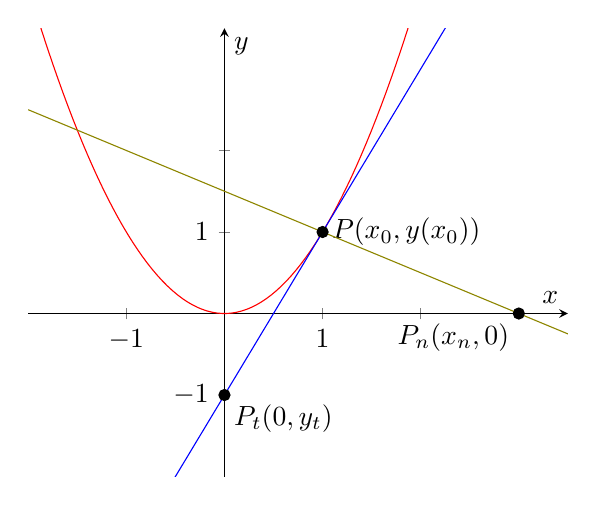
\begin{tikzpicture}
                \begin{axis}[
                    axis lines = center,
                    xlabel = \(x\),
                    ylabel = \(y\),
                    xmin = -2, xmax = 3.5,
                    ymin = -2, ymax = 3.5,
                    xtick = {-1, 1, 2},
                    ytick = {-1, 1, 2},
                    xticklabels = {\(-1\), \(1\)},
                    yticklabels = {\(-1\), \(1\)},
                ]
                \addplot[domain=-2:2, samples=80, color=red]{x^2};

                % Marcamos el punto P(x_0, y(x_0))
                \addplot[mark=*] coordinates {(1, 1)} node[right] {\(P(x_0, y(x_0))\)};

                % Marcamos la recta tangente
                \addplot[domain=-2:3, samples=2, color=blue]{2*x - 1};
                % Marcamos el punto de corte de la recta tangente con el eje de ordenadas
                \addplot[mark=*] coordinates {(0, -1)} node[below right] {\(P_t(0, y_t)\)};

                % Marcamos la recta normal
                \addplot[domain=-2:4, samples=2, color=olive]{-1/2*x + 1.5};
                % Marcamos el punto de corte de la recta normal con el eje de abscisas
                \addplot[mark=*] coordinates {(3, 0)} node[below left] {\(P_n(x_n, 0)\)};
                \end{axis}
            \end{tikzpicture}
            \caption{Representación gráfica del enunciado del Ejercicio~\ref{ej:1.2}.\ref{ej:1.2_b}.}
            \label{fig:ej1.2_b}
        \end{figure}

        Sea el punto \(P=(x_0, y(x_0))\). Para ambas rectas, usaremos la ecuación punto-pendiente. Para la recta tangente, tenemos que:
        \begin{equation*}
            \left. \begin{aligned}
                m_t &= y'(x_0)\\
                P_t &= (0, y_t)
            \end{aligned} \right\} \Longrightarrow y'(x_0) = \dfrac{y(x_0) - y_t}{x_0 - 0}
            \Longrightarrow y_t = y(x_0) - x_0\cdot y'(x_0)
        \end{equation*}
        Notemos además que, en el caso de $x_0=0$, también podemos ver que se cumple que $y_t = y(x_0)-0\cdot y'(x_0) = y(x_0)$. Respecto a la recta normal, tenemos que:
        \begin{equation*}
            \left. \begin{aligned}
                m_n &= -\dfrac{1}{y'(x_0)}\\
                P_n &= (x_n, 0)
            \end{aligned} \right\} \Longrightarrow -\dfrac{1}{y'(x_0)} = \dfrac{0 - y(x_0)}{x_n - x_0}
            \Longrightarrow x_n = y(x_0)\cdot y'(x_0) + x_0
        \end{equation*}
        Notemos que, si $y'(x_0) = 0$, se cumple también que $x_n = 0\cdot y(x_0) + x_0 = x_0$. Además, si $x_n=x_0$, entonces se tiene que $y'(x_0) = 0$ o  $y(x_0)=0$, por lo que también se cumple.

        La ecuación diferencial que especifica el enunciado es $|y_t| = |x_n|$. Por tanto, tenemos que:
        \begin{equation*}
            \left| y(x_0) - x_0\cdot y'(x_0) \right| = \left| y(x_0)\cdot y'(x_0) + x_0 \right|
        \end{equation*}

        Quitando los valores absolutos, llegamos a que:
        \begin{align*}
            y(x_0) - x_0\cdot y'(x_0) = y(x_0)\cdot y'(x_0) + x_0
            &\Longrightarrow y(x_0) - x_0 = y'(x_0)\left( y(x_0) + x_0 \right)\\
            y(x_0) - x_0\cdot y'(x_0) = -y(x_0)\cdot y'(x_0) - x_0
            &\Longrightarrow y(x_0) + x_0 = y'(x_0)\left( x_0 -y(x_0)\right)
        \end{align*}

        Por tanto, describe varias ecuaciones diferenciales distintas:
        \begin{align*}
            y' &= \dfrac{y - x}{y + x} \qquad \text{con dominio } \left\{\begin{array}{c}
                D_1=\{(x, y)\in \bb{R}^2 \mid y<-x\}\\
                \lor \\
                D_2=\{(x, y)\in \bb{R}^2 \mid y>-x\}.\\
            \end{array}\right. \\ \\
            y' &= \dfrac{y+x}{x-y} \qquad \text{con dominio } \left\{\begin{array}{c}
                D_1=\{(x, y)\in \bb{R}^2 \mid y<x\}\\
                \lor \\
                D_2=\{(x, y)\in \bb{R}^2 \mid y>x\}.\\
            \end{array}\right.
        \end{align*}

        % // TODO: Al dividir, no he perdido puntos?
    \end{enumerate}
\end{ejercicio}


\begin{ejercicio}
    En ciertas reacciones químicas, la velocidad a la que se forma un nuevo compuesto viene dada por la ecuación
    \begin{equation*}
        x' = k(x - \alpha)(\beta - x),
    \end{equation*}
    donde \(x(t)\) es la cantidad de compuesto a tiempo \(t\), \(k > 0\) es una constante de proporcionalidad y \(\beta > \alpha > 0\). Usando el campo de direcciones, prediga el comportamiento de \(x(t)\) cuando \(t \to +\infty\).\\

    Del contexto, deducimos que $x\in C^1(\bb{R}^+_0)$. Además, tenemos que su primera derivada solo se anula en $x=\alpha$ y $x=\beta$.
    Consideramos por tanto los siguientes casos:
    \begin{itemize}
        \item \ul{Si $x\in \left]0, \alpha\right[$:} En este caso, $x<\alpha<\beta$, luego $x-\alpha<0$ y $\beta-x>0$. Por tanto, $x'<0$,
        luego es decreciente.
        \item \ul{Si $x\in \left]\alpha, \beta\right[$:} En este caso, $\alpha<x<\beta$, luego $x-\alpha>0$ y $\beta-x>0$. Por tanto, $x'>0$,
        luego es creciente.
        \item \ul{Si $x\in \left]\beta, +\infty\right[$:} En este caso, $x>\beta>\alpha$, luego $x-\alpha>0$ y $\beta-x<0$. Por tanto, $x'<0$,
        luego es decreciente.
    \end{itemize}

    Por tanto, para el comportamiento de $x(t)$ cuando $t\to +\infty$, tenemos que:
    \begin{itemize}
        \item Si $x(0)\in \left]0, \alpha\right[$, entonces $x'$ es decreciente, luego $x(t)\to 0$.
        \item Si $x(0)\in \left]\alpha, \beta\right[$, entonces $x'$ es creciente, luego $x(t)\to \beta$.
        \item Si $x(0)\in \left]\beta, +\infty\right[$, entonces $x'$ es decreciente, luego $x(t)\to \beta$.
    \end{itemize}
\end{ejercicio}


\begin{ejercicio}
    Encuentre la familia de trayectorias ortogonales a las familias de curvas siguientes, teniendo en cuenta que para resolver las ecuaciones que aparecen en \ref{itm:ej1.4_b} y \ref{itm:ej1.4_c} habrá que esperar a la siguiente lección:
    \begin{enumerate}
        \item \(xy = k\),
        
        Buscamos en primer lugar la ecuación diferencial que describe la familia de curvas dada. Para ello, derivamos implícitamente la ecuación dada:
        \begin{equation*}
            0 = y + xy' \Longrightarrow y' = -\dfrac{y}{x}
        \end{equation*}

        Por tanto, tenemos que la familia de curvas dada son las soluciones de dicha ecuación diferencial.
        Sabiendo que el producto de las pendientes ortogonales es $-1$, tenemos que la ecuación diferencial que describe las curvas ortogonales es:
        \begin{equation*}
            y' = \dfrac{x}{y}
        \end{equation*}
        
        \item\label{itm:ej1.4_b} \(y = kx^4\),
        
        Buscamos en primer lugar la ecuación diferencial que describe la familia de curvas dada. Para ello, derivamos implícitamente la ecuación dada:
        \begin{equation*}
            0 = 4kx^3 - y' \Longrightarrow y' = 4kx^3 = 4\cdot \dfrac{y}{x^4} \cdot x^3 = 4\cdot \dfrac{y}{x}
        \end{equation*}

        Por tanto, tenemos que la familia de curvas dada son las soluciones de dicha ecuación diferencial.
        Sabiendo que el producto de las pendientes ortogonales es $-1$, tenemos que la ecuación diferencial que describe las curvas ortogonales es:
        \begin{equation*}
            y' = -\dfrac{x}{4y}
        \end{equation*}
        \item\label{itm:ej1.4_c} \(y = e^{kx}\).
        
        Buscamos en primer lugar la ecuación diferencial que describe la familia de curvas dada. Para ello, derivamos implícitamente la ecuación dada:
        \begin{equation*}
            0 = ke^{kx} - y' \Longrightarrow y' = ke^{kx}
        \end{equation*}

        Para despejar la $k$, tenemos que $k = \dfrac{\ln y}{x}$. Por tanto, tenemos que:
        \begin{equation*}
            y' = \dfrac{\ln y}{x}\cdot e^{\frac{\ln y}{x}\cdot x} = \dfrac{\ln y}{x}\cdot y
        \end{equation*}

        Por tanto, tenemos que la familia de curvas dada son las soluciones de dicha ecuación diferencial.
        Sabiendo que el producto de las pendientes ortogonales es $-1$, tenemos que la ecuación diferencial que describe las curvas ortogonales es:
        \begin{equation*}
            y' = -\dfrac{x}{y \ln y}
        \end{equation*}
    \end{enumerate}
\end{ejercicio}


\begin{ejercicio} \label{ej:1.5}
    Haga un dibujo aproximado del campo de direcciones asociado a la ecuación
    \begin{equation*}
        x' = t + x^3.
    \end{equation*}
    Dibuje la curva donde las soluciones alcanzan un punto crítico. Considerando una solución tal que \(x(0) = 0\), demuestre que tal solución alcanza en 0 un mínimo local estricto y que de hecho es el mínimo global.\\

    Las soluciones alcanzan un punto crítico donde $x'(t)=0$, es decir, $t+x^3=0$. Por tanto, las soluciones alcanzan un punto crítico en la curva $x(t)=\sqrt[3]{-t}$.
    El dibujo, tanto del campo de direcciones como de la curva, se encuentra en la Figura~\ref{fig:ej1.5}.
    \begin{figure}[H]
        \centering
        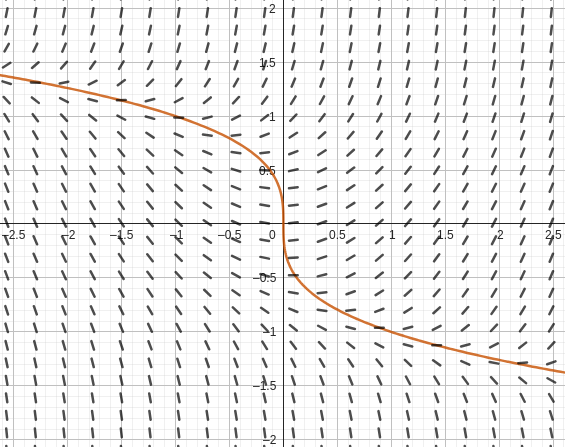
\includegraphics[width=0.5\textwidth]{Imagenes/Rel1_Ej5.png}
        \caption{Campo de direcciones y curva del Ejercicio~\ref{ej:1.5}.}
        \label{fig:ej1.5}
    \end{figure}

    Supongamos ahora una solución tal que $x(0)=0$. Como $x$ es una solución de una ecuación diferencial de primer orden, tenemos que $x\in C^1(\bb{R})$. Por tanto, $x$ es derivable en $0$. Calculamos la derivada de $x$ en $0$:
    \begin{equation*}
        x'(0) = 0 + x(0)^3 = 0
    \end{equation*}

    Por tanto, tenemos que es un punto crítico. Comprobemos que es un mínimo local estricto. Para ello, calculamos la segunda derivada de $x$ en $0$:
    \begin{equation*}
        x''(0) = 1 + 3x(0)^2\cdot x'(0) = 1 + 3\cdot 0^2\cdot 0 = 1 > 0
    \end{equation*}
    Por tanto, es un mínimo local estricto.\\
    
    Respecto de la demostración de que es un mínimo global, intuitivamente observando el campo de direcciones se tiene directamente.
    % // TODO: Formalmente? Cómo demostrar que es mínimo global?
\end{ejercicio}


\begin{ejercicio} Resuelva los siguientes apartados:
    \begin{enumerate}
        \item Estudie cuántas funciones diferenciables \(y(x)\) se pueden extraer de la curva
        \begin{equation*}
            C \equiv x^2 + 2y^2 + 2x + 2y = 1,
        \end{equation*}
        dando su intervalo maximal de definición.

        Buscamos completar cuadrados para obtener las funciones $y(x)$:
        \begin{align*}
            x^2 &+ 2y^2 + 2x + 2y = (x+1)^2 -1 + 2(y^2+y)
            = (x+1)^2 -1+ 2(y^2+y+\nicefrac{1}{4} - \nicefrac{1}{4})
            =\\&= (x+1)^2 -1+ 2(y+\nicefrac{1}{2})^2 - \nicefrac{1}{2}
        \end{align*}
        
        Por tanto, tenemos que:
        \begin{equation*}
            C\equiv (x+1)^2 + 2(y+\nicefrac{1}{2})^2 = \nicefrac{5}{2}
            \equiv (y+\nicefrac{1}{2})^2 = \dfrac{\nicefrac{5}{2} - (x+1)^2}{2}
        \end{equation*}

        Aplicando la raíz cuadrada, tenemos que:
        \begin{equation*}
            y(x) = \pm \sqrt{\dfrac{\nicefrac{5}{2} - (x+1)^2}{2}} - \nicefrac{1}{2}
        \end{equation*}
        Por tanto, vemos que obtenemos dos funciones diferenciables, una para cada signo. Como $C$ es una elipse, se trata de la parte superior e inferior de la misma. El intervalo maximal de definición es aquel que mantiene el argumento de la raíz cuadrada positivo:
        \begin{multline*}
            \dfrac{\nicefrac{5}{2} - (x+1)^2}{2} \geq 0 \Longrightarrow \nicefrac{5}{2} \geq (x+1)^2 \Longrightarrow -\nicefrac{5}{2} \leq x+1 \leq \nicefrac{5}{2} \Longrightarrow |x+1|\leq \sqrt{\nicefrac{5}{2}}
            \Longrightarrow \\ \Longrightarrow
            -\sqrt{\nicefrac{5}{2}}-1 \leq x \leq \sqrt{\nicefrac{5}{2}}-1
        \end{multline*}

        Por tanto, el intervalo maximal de definición es $I=\left[-\sqrt{\nicefrac{5}{2}}-1, \sqrt{\nicefrac{5}{2}}-1\right]$.
        \item Usando derivación implícita, encuentre una ecuación diferencial de la forma \(y' = f(x, y)\) que admita como soluciones a las funciones del apartado anterior.
        
        Derivamos implícitamente la ecuación dada:
        \begin{equation*}
            2x +2+(4y+2)y' = 0 \Longrightarrow y' = -\dfrac{2x+2}{4y+2} = -\dfrac{x+1}{2y+1}
        \end{equation*}

        Por tanto, la ecuación diferencial que describe las funciones del apartado anterior es $y=f(x, y)$, con:
        \begin{equation*}
            f(x, y) = -\dfrac{x+1}{2y+1} \qquad \text{con dominio } \left\{\begin{array}{c}
                D_1=\{(x, y)\in \bb{R}^2 \mid 2y+1>0\}\\
                \lor \\
                D_2=\{(x, y)\in \bb{R}^2 \mid 2y+1<0\}.\\
            \end{array}\right.
        \end{equation*}
        \item La misma cuestión para una ecuación del tipo \(g(y, y') = 0\).
        
        % // TODO: ¿Cómo se hace?
    \end{enumerate}
\end{ejercicio}


\begin{ejercicio} \label{ej:1.7}
    Una persona, partiendo del origen, se mueve en la dirección del eje \(x\) positivo tirando de una cuerda de longitud \(s\) atada a una piedra.
    Se supone que la cuerda se mantiene tensa en todo momento, y que la piedra es arrastrada desde el punto de partida \((0, s)\).
    La trayectoria que describe la piedra es una curva clásica llamada tractriz.
    Encuentre una ecuación diferencial para la misma.
    \begin{observacion}
        Se supone que la cuerda se mantiene tangente a la trayectoria de la piedra en todo momento.
    \end{observacion}

    La situación descrita se encuentra en la Figura~\ref{fig:ej1.7}.
    \begin{figure}[H]
        \centering
        \begin{tikzpicture}
            \begin{axis}[
                axis lines = center,
                xlabel = \(x\),
                ylabel = \(y\),
                xmin = -1, xmax = 4,
                ymin = -1, ymax = 4
            ]
            \addplot[domain=0:4, samples=100, color=red]{1/(x+0.4)};

            % Marca del (0,s)
            \addplot[mark=*] coordinates {(0, 2.5)} node[above right] {\((0, s)\)};

            % Recta tangente a la curva en (1,f(1))
            \addplot[domain=1:2.4, samples=2, color=blue]{(-1/(1+0.4)^2)*(x-1)+1/(1+0.4)} node[midway, left] {\(s\)};

            % Marca del punto (1,f(1))
            \addplot[mark=*] coordinates {(1, 0.714285)} node[above right] {\(P(x, y(x))\)};

            % Marca del punto (x,0)
            \addplot[mark=*] coordinates {(2.4, 0)} node[below, yshift=-1em] {\(P_t(x_t, 0)\)};
            \end{axis}
        \end{tikzpicture}
        \caption{Representación gráfica de la situación del Ejercicio~\ref{ej:1.7}.}
        \label{fig:ej1.7}
    \end{figure}

    Por tanto, la condición impuesta es que la distancia desde un punto de la gráfica al punto de corte de la tangente a la curva por ese punto con el eje de abscisas es constante e igual a $s$. Es decir, si el punto es \((x, y(x))\), entonces la condición es:
    \begin{equation*}
        \sqrt{(x-x_t)^2 + y(x)^2} = s
    \end{equation*}

    Veamos cómo calcular $x_t$. Usando la definición de pendiente con los puntos $P$ y $P_t$, tenemos:
    \begin{equation*}
        y'(x) = \dfrac{y(x) - 0}{x - x_t} \Longrightarrow x_t = x - \dfrac{y(x)}{y'(x)}
    \end{equation*}

    Notemos que $y'(x)=0$ no tiene sentido, puesto que la recta descrita sea horizontal, y por tanto no habría punto de corte con el eje $X$ (es decir, no habría un único $x_t$). Por tanto, la ecuación diferencial que describe la curva es:
    \begin{equation*}
        \sqrt{\left(x-x + \dfrac{y(x)}{y'(x)}\right)^2 + y(x)^2} = s
        \Longrightarrow
        \sqrt{\dfrac{y(x)^2}{y'(x)^2} + y(x)^2} = s
    \end{equation*}

    Elevando al cuadrado, tenemos que:
    \begin{equation*}
        \dfrac{y(x)^2}{y'(x)^2} + y(x)^2 = s^2
        \Longrightarrow
        y'(x)^2 = \dfrac{y(x)^2}{s^2 - y(x)^2}
    \end{equation*}

    Notemos que $y(x)<s$ para todo $x\in \bb{R}$, por lo que el denominador es siempre positivo. Aplicamos ahora la raíz cuadrada, sabiendo que $y'(x)<0$ por ser la pendiente de la curva decreciente, y $y(x)>0$ para todo $x\in \bb{R}$:
    \begin{equation*}
        y'(x) = -\dfrac{y(x)}{\sqrt{s^2 - y(x)^2}}
    \end{equation*}

    Usando la notación correspondiente, tenemos que la ecuación diferencial que describe la curva es:
    \begin{equation*}
        y' = -\dfrac{y}{\sqrt{s^2 - y^2}} \qquad \text{ con dominio } D=\{(x, y)\in \bb{R}^2 \mid -s<y<s\}
    \end{equation*}
\end{ejercicio}


\begin{ejercicio}
    Demuestre que si \(x(t)\) es una solución de la ecuación diferencial
    \begin{equation}\label{eq:ej1.8_1}
        x'' + x = 0,
    \end{equation}
    entonces también cumple, para alguna constante \(c \in \bb{R}\),
    \begin{equation}\label{eq:ej1.8_2}
        (x')^2 + x^2 = c.
    \end{equation}

    Encuentre una solución de $(x')^2 + x^2 = 1$ que no sea solución de \eqref{eq:ej1.8_1}.\\

    \begin{proof}
        Sea $I\subset \bb{R}$ el intervalo de definición de $x(t)$ solución de \eqref{eq:ej1.8_1}. Definimos la función auxiliar
        \Func{f}{I}{\bb{R}}{t}{(x'(t))^2 + x^2(t).}

        Por ser $x$ una solición de una ecuación diferencial de segundo orden, tenemos que $x\in C^2(I)$. Por tanto, $x,~x'\in C^1(I)$ y, por tanto $f$ es derivable. Calculamos su derivada:
        \begin{equation*}
            f'(t) = 2x'(t)x''(t) + 2x(t)x'(t) = 2x'(t)~\left[ x''(t) + x(t) \right] = 2x'(t)\cdot 0 = 0.
        \end{equation*}

        Por tanto, $f'(t)=0$ para todo $t\in I$, lo que implica que $f$ es constante en $I$. Es decir, existe $c\in \bb{R}$ tal que
        \begin{equation*}
            (x'(t))^2 + x^2(t) = c \quad \forall t\in I.
        \end{equation*}

        Por tanto, queda demostrado lo pedido.
    \end{proof}

    Para la segunda parte, sea la solución $x(t) = 1$ para todo $t\in \bb{R}$. Entonces, tenemos que:
    \begin{align*}
        (x'(t))^2 + x^2(t) &= 0^2 + 1^2 = 1,\\
        x''(t) + x(t) &= 0 + 1 = 1
    \end{align*}
\end{ejercicio}



\begin{ejercicio} \label{ej:1.9}
    Una nadadora intenta atravesar un río pasando de la orilla \(y = -1\) a la orilla opuesta \(y = 1\).
    La corriente es uniforme, con velocidad \(v_R > 0\) y paralela a la orilla.
    Por otra parte, la nadadora se mueve a velocidad constante \(v_N > 0\) y apunta siempre hacia una torre situada en el punto \(T = (2, 1)\).
    Las ecuaciones
    \begin{align*}
        \dfrac{dx}{dt} &= v_R + v_N \cdot \dfrac{2 - x}{\sqrt{(2 - x)^2 + (1 - y)^2}},\\
        \dfrac{dy}{dt} &= v_N \cdot \dfrac{1 - y}{\sqrt{(2 - x)^2 + (1 - y)^2}},
    \end{align*}
    describen la posición \((x, y)\) de la nadadora en el instante \(t\); es decir \(x = x(t)\), \(y = y(t)\).
    \begin{enumerate}
        \item Explique cómo se ha obtenido este sistema.
        
        Representemos la situación en la Figura~\ref{fig:ej1.9}.
        \begin{figure}[H]
            \centering
            \begin{tikzpicture}
                \begin{axis}[
                    axis lines = center,
                    xlabel = \(x\),
                    ylabel = \(y\),
                    xmin = -2, xmax = 4,
                    ymin = -2, ymax = 2,
                    xtick = {2},
                    ytick = {1},
                    xticklabels = {\(2\)},
                    yticklabels = {\(1\)},
                ]
                \addplot[domain=-2:4, samples=2, color=red]{1};
                \addplot[domain=-2:4, samples=2, color=red]{-1};
                \addplot[mark=*] coordinates {(2, 1)} node[above right] {\(T(2, 1)\)};

                % Marcamos el punto P(x(t), y(t))
                \addplot[mark=*] coordinates {(0.5, -0.5)} node[below left] {\(P(x(t), y(t))\)};

                % Marcamos la velocidad v_R y v_N
                \draw[-Stealth] (0.5, -0.5) -- (1.7, -0.5) node[midway, below] {\(v_R\)};
                \draw[-Stealth] (0.5, -0.5) -- (1.5,0.5) node[midway, above left] {\(v_N\)};

                % Ángulo alpha entre v_N y v_R
                \draw[blue] (0.9, -0.5) arc (0:45:0.4) node[right] {\(\alpha\)};

                % Triángulo rectángulo con hipotenusa PT
                \draw[dashed] (0.5, -0.5) -- (2, 1) -- (2, -0.5) -- cycle;
                \end{axis}
            \end{tikzpicture}
            \caption{Representación gráfica de la situación del Ejercicio~\ref{ej:1.9}.}
            \label{fig:ej1.9}
        \end{figure}
        
        Tenemos que $x(t)$ es la componente horizontal de la posición de la nadadora, por lo que $x'(t)$ es la velocidad horizontal de la nadadora:
        \begin{equation*}
            x'(t) = v_R + v_N \cdot \cos(\alpha) \AstIg
            v_R + v_N \cdot \dfrac{2 - x}{\sqrt{(2 - x)^2 + (1 - y)^2}}
        \end{equation*}
        donde en $(\ast)$ hemos empleado la definición de coseno como cateto contiguo sobre hipotenusa. Por otro lado, $y(t)$ es la componente vertical de la posición de la nadadora, por lo que $y'(t)$ es la velocidad vertical de la nadadora:
        \begin{equation*}
            y'(t) = v_N \cdot \sen(\alpha) \AstIg v_N \cdot \dfrac{1 - y}{\sqrt{(2 - x)^2 + (1 - y)^2}}
        \end{equation*}
        donde en $(\ast)$ hemos empleado la definición de seno como cateto opuesto sobre hipotenusa.
        
        \item Encuentre la ecuación diferencial de la órbita \(y = y(x)\).
        
        Tenemos que:
        \begin{equation*}
            \dfrac{dy}{dx} = \dfrac{\nicefrac{dy}{dt}}{\nicefrac{dx}{dt}} = \dfrac{v_N \cdot \dfrac{1 - y}{\sqrt{(2 - x)^2 + (1 - y)^2}}}{v_R + v_N \cdot \dfrac{2 - x}{\sqrt{(2 - x)^2 + (1 - y)^2}}}
            = \dfrac{1-y}{\dfrac{v_R}{v_N}\sqrt{(2 - x)^2 + (1 - y)^2} + 2-x}
        \end{equation*}
    \end{enumerate}
\end{ejercicio}


\begin{ejercicio}
    Encuentre una ecuación diferencial de segundo orden que admita como soluciones a las siguientes familias de funciones, donde \(c_1, c_2 \in \bb{R}\):
    \begin{enumerate}
        \item \(x = c_1e^t + c_2e^{-t}\),
        
        Derivamos dos veces:
        \begin{align*}
            x' &= c_1e^t - c_2e^{-t},\\
            x'' &= c_1e^t + c_2e^{-t}.
        \end{align*}

        Como conclusión, vemos que la ecuación diferencial $x''=x$ con dominio $D=\bb{R}^2$ admite como solución a la familia de funciones dada.
        \item \(x = c_1\cosh t + c_2\senh t\).
        
        Derivamos dos veces:
        \begin{align*}
            x' &= c_1\senh t + c_2\cosh t,\\
            x'' &= c_1\cosh t + c_2\senh t.
        \end{align*}

        Como conclusión, vemos que la ecuación diferencial $x''=x$ con dominio $D=\bb{R}^2$ admite de nuevo como solución a la familia de funciones dada.
    \end{enumerate}
\end{ejercicio}


\begin{ejercicio}
    Dada la ecuación de Clairaut:
    \begin{equation*}
        x = tx' + \varphi(x')
    \end{equation*}
    \begin{enumerate}
        \item Encuentre una familia uniparamétrica de soluciones rectilíneas.
        % // TODO: ¿Cómo se hace?
        \item Suponiendo que \(\varphi(x) = x^2\), demuestre que \(x(t) = -\dfrac{t^2}{4}\) también es solución.
        
        Para esto, vemos:
        \begin{equation*}
            tx'+\varphi(x') = t\cdot \left(\dfrac{-2t}{4}\right) + \left(\dfrac{-2t}{4}\right)^2 = -\dfrac{t^2}{2} + \dfrac{t^2}{4} = -\dfrac{t^2}{4} = x
        \end{equation*}
        Por tanto, \(x(t) = -\dfrac{t^2}{4}\) es solución.
        \item ¿Qué relación hay entre esta solución y las que se han encontrado antes?
    \end{enumerate}
\end{ejercicio}

\begin{ejercicio}
    Resuelva los problemas 6 y 7 de la página 33 (sección 2.6) del libro de Ahmad-Ambrosetti.

    \begin{enumerate}
        \item \textbf{Problema 6:} Transformar la ecuación $e^{x'}=x$ en una ecuación en forma normal y prueba que tiene una única solución tal que $x(t_0)=a$ para todo $t_0$ y todo $a\in \bb{R}^+$.
        
        Aplicando el logaritmo neperiano, tenemos que la ecuación diferencial en forma normal es:
        \begin{equation*}
            x' = \ln x\qquad \text{con dominio } D=\bb{R}\times \bb{R}^+
        \end{equation*}

        % // TODO: Unicidad
        
        \item \textbf{Problema 7:} Encuentra la ecuación cuya solución es la catenaria:
        \begin{equation*}
            x(t) = \cosh\left(t\right) = \dfrac{e^t + e^{-t}}{2}
        \end{equation*}

        Calculamos su derivada:
        \begin{equation*}
            x'(t) = \dfrac{e^t - e^{-t}}{2} = \senh(t)
        \end{equation*}

        Por tanto, la ecuación diferencial que describe la catenaria es:
        \begin{equation*}
            x' = \senh(t) \qquad \text{con dominio } D=\bb{R}^2
        \end{equation*}
    \end{enumerate}
\end{ejercicio}

